\subsection{Polimorfizmus az objektum-orientált programozásban. Virtuális alaposztályok. Abstract osztály. Általánosított osztályok.}

\textbf{Öröklődés:}
\begin{itemize}
    \item egy osztály felhasználható arra, hogy egy új, leszármazott osztályt hozzunk létre belőle
    \item hierarchia alakítható ki
    \item leszármazottban benne van az ősosztály összes adattagja és metódusa
    \item plusz adattagokkal és metódusokkal bővíthető
    \item adattagot, metódust törölni nem lehet
    \item ősben lévő kód újrahasznosul, nem kell újra megírni
    \item az ős változtatása benne lesz a leszármazottban is
    \item a meglévő kód bővíthető és változtatható is
    \item \texttt{protected} tagok: maradjon meg az adatrejtés elve, de a leszármazottak el tudják érni az ős adatait
    \item öröklődnek:
    \begin{itemize}
        \item metódusok, adattagok, operátorok
    \end{itemize}
    \item nem öröklődnek:
    \begin{itemize}
        \item konstruktorok
        \item destruktorok
        \item barát függvények
        \item túlterhelt = operátor
    \end{itemize}
\end{itemize}

\textbf{Sokalakúság:}
\begin{itemize}
    \item az örökléssel létrehozott osztály máshogy viselkedhet, mint az ősosztály
    \item megvalósítás: ugyanolyan nevű és paraméterű metódust tartalmaz, a törzsében más utasításokkal
\end{itemize}

\textbf{Polimorfizmus:}
\begin{itemize}
    \item a leszármazott osztály máshogy viselkedik mint az ős
    \item úgy érjük el, hogy az ugyanolyan nevű és paraméterű metódusát felülírjuk
    \item nem overload, hiszen a paramétereken nem változtatunk
    \item \texttt{override}: felülírás
    \item példa:
\end{itemize}

\begin{minipage}{0.5\textwidth}
\begin{minted}{cpp}
class p2d
{
    double x, y;
public:
    // konstruktor, get(), <<
    double tavolsag()
    {
        return sqrt(pow(x, 2) + pow(y, 2));
    }
};

class p3d :public p2d
{
    double z;
public:
    // konstuktor, get(), <<
    double tavolsag()
    { // x és y csak get_tel. protected-del is működne!
        return sqrt(pow(get_x(), 2) + pow(get_y(), 2) +
                pow(z, 2));
    }
};
\end{minted}
\end{minipage}%
\begin{minipage}{0.5\textwidth}
    \centering
    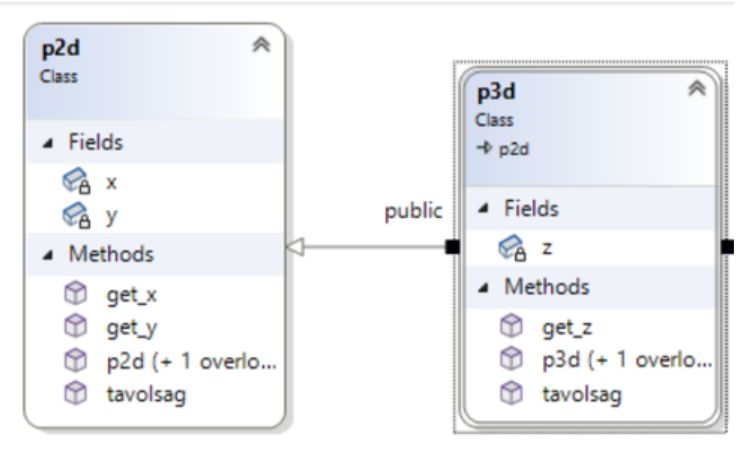
\includegraphics[width=\textwidth]{res/imgs/info_14_polymorphism.png}
\end{minipage}

\begin{minted}{cpp}
p2d p1(1, 1);
p3d p2(2, 2, 2);
cout << "p1 az origotol:" << p1.tavolsag() << endl;
cout << "p2 az origotol:" << p2.tavolsag() << endl;
p1 = p2; // minden leszármazottban benne van az ős. z-t kidobjuk! C++ Core Guidelines: ES.63: Don't slice
cout << "p1: " << p1 << endl;
cout << "p1 az origotol:" << p1.tavolsag() << endl;
\end{minted}

\textbf{Korai kötés:}
\begin{itemize}
    \item alaphelyzeten a metódusok fordítás közben bekerülnek az osztályba
    \item híváskor a fordítás közben megkapott címet használjuk
    \item ha a leszármazottat ősosztály típussal használjuk, akkor az ős metódusa fog lefutni a leszármazott adataival
    \item ez a módszer a korai kötés
\end{itemize}

\textbf{Virtuális metódusok:}
\begin{itemize}
    \item a \texttt{virtual} kulcsszó jelzi a fordítónak, hogy ezt a metódust ne drótozza be az osztályba
    \item készít egy táblázatot, ahol a metódusok címei szerepelnek
    \item futás közben ez a táblázat aktualizálódik
    \item a futás közben kiderülő függvénycímek miatt ezt a módszert késői kötésnek nevezzük
    \item ha egy metódus az ősben virtuális volt, a leszármazottban is az lesz, felülírás esetén is
    \item \texttt{override} kiírható, de nem kötelező
\end{itemize}

\textbf{VMT:}
\begin{itemize}
    \item Virtuális Metódusok Táblája (vftable)
    \item a példányhoz tartozó VMT tartalmazza a virtuális metódusokat
    \item \texttt{vpointer}: VMT-re mutató pointer
    \begin{itemize}
        \item direktben nem látjuk
    \end{itemize}
\end{itemize}

\textbf{Tisztán virtuális metódus:}
\begin{itemize}
    \item készíthető olyan virtuális metódus, melynek nincs törzse
    \item \texttt{=0} -- val jelöljük, hogy ebben az osztályban nem lesz kifejtve
    \item törzs nélküli metódus: tisztán virtuális metódus
    \item csak virtuális metódus lehet 0-ra végződő
    \item az \texttt{=0} helyett \texttt{abstract} is írható
\end{itemize}

\textbf{Abstract osztály:}
\begin{itemize}
    \item ha az osztály tartalmaz legalább egy tisztán virtuális metódust
    \item nem példányosítható
\end{itemize}

\textbf{Általános osztály:}
\begin{itemize}
    \item nem konkrét objektumot ír le, hanem általános típust
    \item más osztályok őseként szolgál
    \item absztrakt is lehet, ha szükséges
    \item pl.\ abstract class alakzatok -> class négyzet, class kör
\end{itemize}